\documentclass[aspectratio=169,11pt]{beamer}
\usepackage[T1]{fontenc}
\usepackage{lmodern,amsmath,amssymb,mathtools,bm,booktabs,array,graphicx,tikz}
\usetikzlibrary{arrows.meta,positioning,calc,decorations.pathreplacing,patterns}
\definecolor{ink}{HTML}{17344D}\definecolor{accent}{HTML}{087E8B}\definecolor{pale}{HTML}{EDF5F5}\definecolor{gold}{HTML}{AD6B19}
\providecommand{\dd}{\,\mathrm{d}}\providecommand{\R}{\mathbb{R}}
\providecommand{\E}{\mathbb{E}}\providecommand{\Var}{\operatorname{Var}}
\providecommand{\Cov}{\operatorname{Cov}}\providecommand{\diag}{\operatorname{diag}}
\providecommand{\norm}[1]{\left\lVert#1\right\rVert}
\providecommand{\abs}[1]{\left|#1\right|}
\usefonttheme{professionalfonts}
\setbeamercolor{normal text}{fg=black,bg=white}
\setbeamercolor{frametitle}{fg=ink,bg=white}
\setbeamercolor{title}{fg=ink}\setbeamercolor{structure}{fg=accent}
\setbeamercolor{block title}{fg=ink,bg=pale}\setbeamercolor{block body}{fg=black,bg=pale!40}
\setbeamercolor{alerted text}{fg=accent}
\setbeamerfont{frametitle}{size=\Large,series=\bfseries}
\setbeamerfont{title}{size=\LARGE,series=\bfseries}
\setbeamertemplate{navigation symbols}{}
\setbeamersize{text margin left=.7cm,text margin right=.7cm}
\setbeamertemplate{frametitle}{\vspace{.18cm}\insertframetitle\par\vspace{.1cm}{\color{accent}\hrule height .6pt}\vspace{.12cm}}
\newcommand{\notestarget}{notes.pdf}\newcommand{\noteslabel}{Notes}
\setbeamertemplate{footline}{\hspace{.7cm}\color{ink}\scriptsize Computational Cardiology\quad\href{\notestarget}{\noteslabel}\hfill\insertframenumber\,/\,\inserttotalframenumber\hspace{.7cm}\vspace{.18cm}}
\setbeamercovered{invisible}
\hypersetup{pdfauthor={Zan Ahmad},pdftitle={Local convolutional segmentation and geometric error},pdfpagemode=UseNone}
\begin{document}
\begin{frame}[plain]\vfill
{\small\color{accent} Computational Cardiology \quad Lecture 12}\par\medskip
{\raggedright\hyphenpenalty=10000\exhyphenpenalty=10000\LARGE\bfseries\color{ink} Local convolutional segmentation and geometric error}\par\bigskip
Zan Ahmad\par\smallskip
{\small Fall 2024}\par\vfill\end{frame}
\renewcommand{\notestarget}{notes.pdf\#note-pixelwise-prediction-and-comparison-units}
\begin{frame}[t,fragile,label=slide-the-output-of-segmentation]{The output of segmentation}
\[I\longmapsto\widehat M\in\{0,1\}^{H\times W}.\]\pause{} A spatial mask contains boundary and connectivity information absent from one image-level label.
\end{frame}
\renewcommand{\notestarget}{notes.pdf\#note-a-shared-local-linear-predictor}
\begin{frame}[t,fragile,label=slide-a-local-shared-predictor]{A local shared predictor}
\[z_i=w^{\mathsf T}x_i+b,\qquad p_i=\sigma(z_i).\]\pause{} The $3\times3$ patch supplies nine weights and one shared bias.
\end{frame}
\renewcommand{\notestarget}{notes.pdf\#note-a-shared-local-linear-predictor}
\begin{frame}[t,fragile,label=slide-the-sigmoid-decision]{The sigmoid decision}
\[\sigma(z)=\frac1{1+e^{-z}},\qquad\widehat y_i=\boldsymbol1_{\{p_i\ge.5\}}.\]\pause{} With threshold $.5$, the class boundary is $z_i=0$.
\end{frame}
\renewcommand{\notestarget}{notes.pdf\#note-a-shared-local-linear-predictor}
\begin{frame}[t,fragile,label=slide-receptive-field-and-padding]{Receptive field and padding}
The rule uses only a $3\times3$ neighborhood. Reflect padding supplies border context.\pause{} A distant anatomical relationship lies outside this receptive field.
\end{frame}
\renewcommand{\notestarget}{notes.pdf\#note-cross-entropy-and-its-derivatives}
\begin{frame}[t,fragile,label=slide-binary-cross-entropy-from-logits]{Binary cross-entropy from logits}
\[J=\frac1M\sum_i[\log(1+e^{z_i})-y_i z_i]+\frac\lambda2\|w\|^2.\]\pause{} A stable log-add-exp evaluation avoids taking logarithms of rounded probabilities.
\end{frame}
\renewcommand{\notestarget}{notes.pdf\#note-cross-entropy-and-its-derivatives}
\begin{frame}[t,fragile,label=slide-differentiate-the-data-term]{Differentiate the data term}
\[\frac{\partial\ell_i}{\partial z_i}=p_i-y_i.\]\pause{}\[\nabla_wJ=\frac1M X^{\mathsf T}(p-y)+\lambda w,\quad\partial_bJ=\frac1M\boldsymbol1^{\mathsf T}(p-y).\]
\end{frame}
\renewcommand{\notestarget}{notes.pdf\#note-cross-entropy-and-its-derivatives}
\begin{frame}[t,fragile,label=slide-curvature-of-the-local-model]{Curvature of the local model}
\[\nabla^2\ell=\frac1M\widetilde X^{\mathsf T}\operatorname{diag}(p_i(1-p_i))\widetilde X\succeq0.\]\pause{} The single-layer objective is convex; weight sharing does not make it a deep network.
\end{frame}
\renewcommand{\notestarget}{notes.pdf\#note-cross-entropy-and-its-derivatives}
\begin{frame}[t,fragile,label=slide-a-gradient-update]{A gradient update}
\[w^{k+1}=w^k-\eta\nabla_wJ,\qquad b^{k+1}=b^k-\eta\partial_bJ.\]\pause{} Validation chooses among saved iterates without using the test set.
\end{frame}
\renewcommand{\notestarget}{notes.pdf\#note-image-level-splitting-and-model-selection}
\begin{frame}[label=slide-the-unit-of-separation-panel-1]{Synthetic test image}
\centering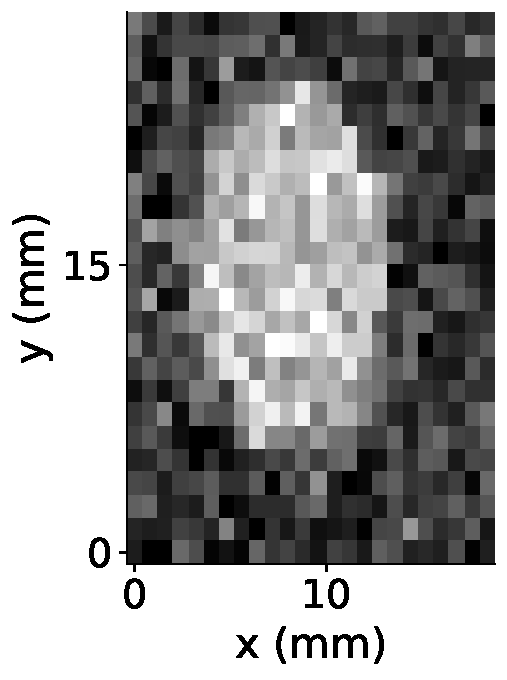
\includegraphics[width=.98\linewidth,height=.69\textheight,keepaspectratio]{presentation-figures/segmentation-comparison-panel-1.pdf}\end{frame}
\renewcommand{\notestarget}{notes.pdf\#note-image-level-splitting-and-model-selection}
\begin{frame}[label=slide-the-unit-of-separation-panel-2]{Generator reference}
\centering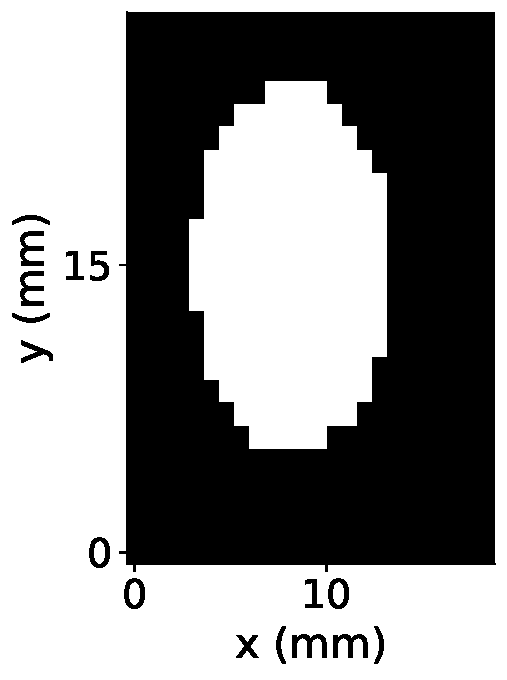
\includegraphics[width=.98\linewidth,height=.69\textheight,keepaspectratio]{presentation-figures/segmentation-comparison-panel-2.pdf}\end{frame}
\renewcommand{\notestarget}{notes.pdf\#note-image-level-splitting-and-model-selection}
\begin{frame}[label=slide-the-unit-of-separation-panel-3]{Fixed threshold 0.5}
\centering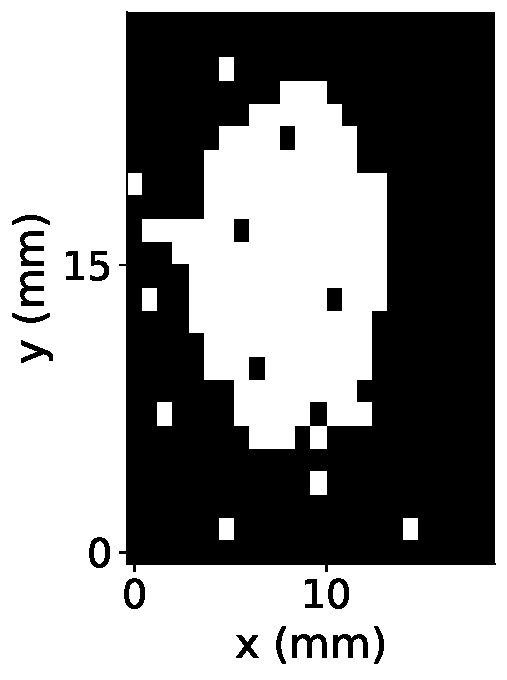
\includegraphics[width=.98\linewidth,height=.69\textheight,keepaspectratio]{presentation-figures/segmentation-comparison-panel-3.pdf}\end{frame}
\renewcommand{\notestarget}{notes.pdf\#note-image-level-splitting-and-model-selection}
\begin{frame}[label=slide-the-unit-of-separation-panel-4]{Learned 3$\times$3 +\allowbreak{} sigmoid}
\centering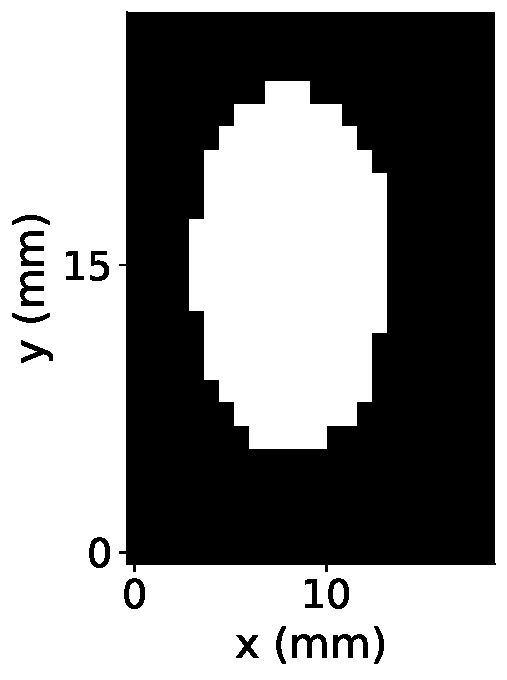
\includegraphics[width=.98\linewidth,height=.69\textheight,keepaspectratio]{presentation-figures/segmentation-comparison-panel-4.pdf}\end{frame}
\renewcommand{\notestarget}{notes.pdf\#note-image-level-splitting-and-model-selection}
\begin{frame}[t,fragile,label=slide-the-unit-of-separation]{The unit of separation}
Complete generated images remain in one split.\pause{} Neighboring patches from one image share both pixels and geometry; splitting pixels would answer an easier prediction problem.
\end{frame}
\renewcommand{\notestarget}{notes.pdf\#note-overlap-boundary-distance-and-topology}
\begin{frame}[t,fragile,label=slide-overlap-as-a-set-quantity]{Overlap as a set quantity}
\[\operatorname{Dice}(P,R)=\frac{2|P\cap R|}{|P|+|R|}.\]\pause{} Equal overlap need not imply equal physical boundary error.
\end{frame}
\renewcommand{\notestarget}{notes.pdf\#note-overlap-boundary-distance-and-topology}
\begin{frame}[t,fragile,label=slide-physical-boundary-distance]{Physical boundary distance}
Compute nearest-boundary distances in both directions using physical coordinates.\pause{} Average distance describes typical displacement; Hausdorff distance records the largest nearest-boundary discrepancy.
\end{frame}
\renewcommand{\notestarget}{notes.pdf\#note-overlap-boundary-distance-and-topology}
\begin{frame}[t,fragile,label=slide-empty-set-conventions]{Empty-set conventions}
Two empty masks have Dice one in this implementation. One empty mask has Dice zero.\pause{} Boundary distance is unavailable when only one boundary is empty.
\end{frame}
\renewcommand{\notestarget}{notes.pdf\#note-overlap-boundary-distance-and-topology}
\begin{frame}[label=slide-a-nearly-perfect-overlap-can-sever-a-bridge-panel-1]{Reference: 1 component}
\centering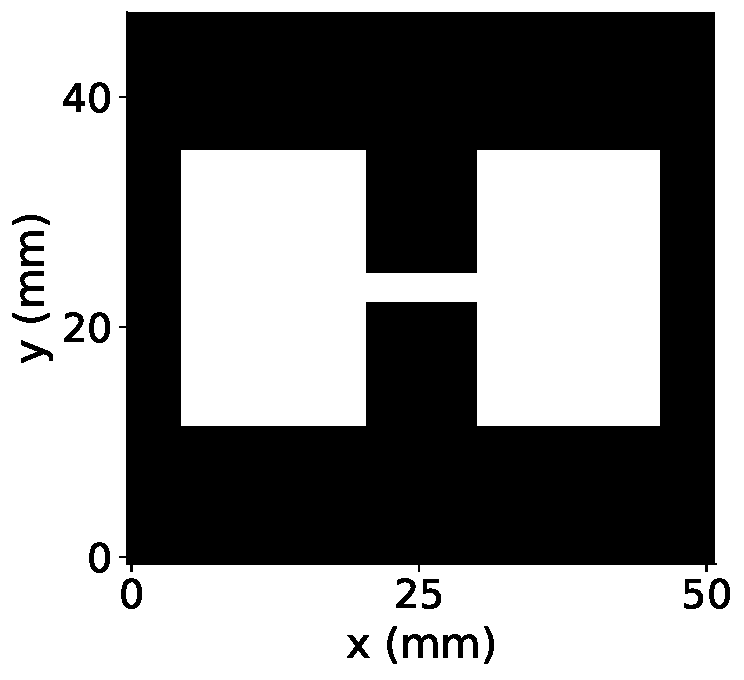
\includegraphics[width=.98\linewidth,height=.69\textheight,keepaspectratio]{presentation-figures/connectivity-failure-panel-1.pdf}\end{frame}
\renewcommand{\notestarget}{notes.pdf\#note-overlap-boundary-distance-and-topology}
\begin{frame}[label=slide-a-nearly-perfect-overlap-can-sever-a-bridge-panel-2]{Four missing pixels: 2 components}
\centering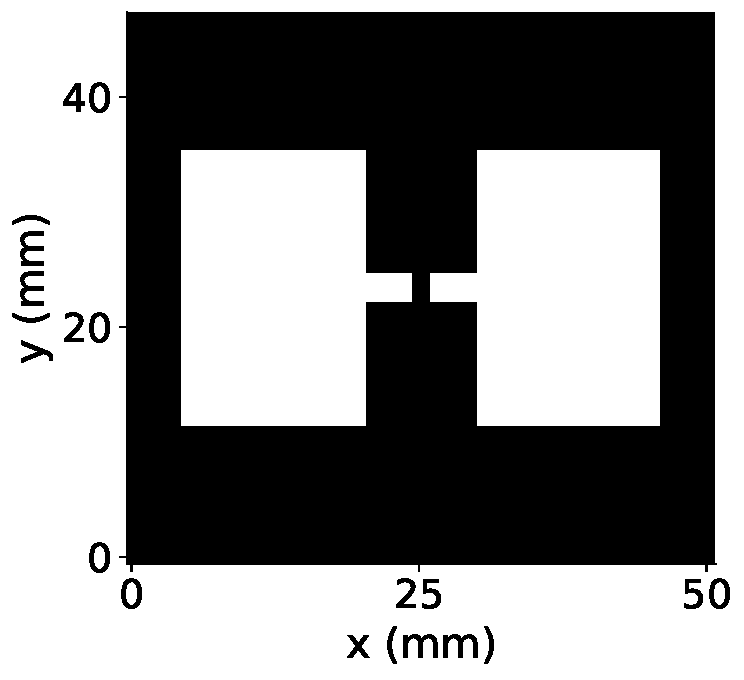
\includegraphics[width=.98\linewidth,height=.69\textheight,keepaspectratio]{presentation-figures/connectivity-failure-panel-2.pdf}\end{frame}
\renewcommand{\notestarget}{notes.pdf\#note-overlap-boundary-distance-and-topology}
\begin{frame}[t,fragile,label=slide-a-nearly-perfect-overlap-can-sever-a-bridge]{A nearly perfect overlap can sever a bridge}
\[|R|=824,\quad|P|=820,\quad\operatorname{Dice}=\frac{1640}{1644}\approx.99757.\]\pause{} Four deleted bridge pixels change one connected component into two.
\end{frame}
\renewcommand{\notestarget}{notes.pdf\#note-the-geometric-consequence-of-a-segmentation-error}
\begin{frame}[t,fragile,label=slide-area-bias-and-overlap-are-distinct]{Area bias and overlap are distinct}
\[e_A=\frac{A_P-A_R}{A_R}.\]\pause{} A signed mean can conceal cancellation of over- and under-segmentation across cases.
\end{frame}
\renewcommand{\notestarget}{notes.pdf\#note-the-geometric-consequence-of-a-segmentation-error}
\begin{frame}[t,fragile,label=slide-the-downstream-geometric-requirement]{The downstream geometric requirement}
A transport model depends on the paths and boundaries of its domain.\pause{} An overlap score cannot by itself certify preservation of those paths.
\end{frame}
\end{document}
